\section{Procesi}
\subsection*{Proces}
Proces je program u izvršavanju zajedno sa svojim virtualnim adresnim prostorom. Svaki proces ima pridružene i sljedeće vrijednosti:
\begin{itemize}
 \item ID procesa (PID)
 \item ID roditelja (PPID)
 \item ID korisnika i grupe
 \item environment varijable
 \item listu otvorenih datoteka
 \item tekući direktorij
 \item itd.
\end{itemize}
\subsection*{Pokretanje procesa}
Svaki proces je pokrenut od strane nekog drugog procesa. Jedini izuzetak je \textbf{init} proces koji pokreće kernel i ima PID 1. Sam \texttt{shell} je proces i njegov \texttt{PID} se može dobiti s: \texttt{echo \$\$}

Iz ljuske se procesi pokreću izvršavanjem komandne linije. Npr. u komandnoj liniji napišite \texttt{bash}. Otvoriti će se subshell. 

\begin{zadatak} Izvršite sljedeće akcije:
\begin{itemize} 
 \item Naći \texttt{PID} aktivne ljuske. Izvršiti naredbu \texttt{history}.
 \item Pokrenite novi \texttt{bash} shell
 \item Naći PID novootvorenog subshella. Izvršiti naredbu \texttt{history}. Što zaključujete?
 \item Izaći iz novootvorenog shella naredbom \texttt{exit}. Provjeriti \texttt{PID} shella u kojem se nalazite. 
\end{itemize}
  
\end{zadatak}
\begin{center} 
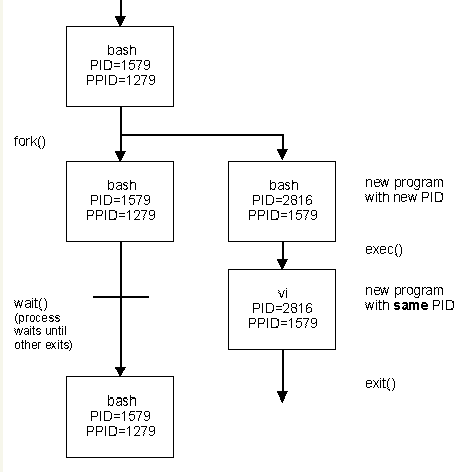
\includegraphics[scale=0.5]{fork.png}%
\end{center}

Procesi se mogu izvršavati na dva načina:
\begin{itemize}
	\item procesi u prednjem planu (eng. \textit{foreground})
	\item procesi u pozadini (eng. \textit{background})
\end{itemize}
\todo[inline]{Je li ovakav prijevod OK?}
Kada se proces izvršava u prednjem planu, ljuska koja ga je pokrenula treba čekati da proces završi kako bi se mogli pokretati ostali procesi. S druge strane, kada se proces izvršava kao pozadinski, ljuska ne mora čekati završetak procesa (odzivni znak se odmah pojavi). Pozadinski procesi se pokreću tako da se na kraj komandne linije doda znak ampersand (\texttt{\&}).

Prebacivanje procesa iz prednjeg plana u pozadinu:
\begin{enumerate}
 \item Suspendirati proces (Ctrl+z)
 \item Unijeti naredbu \texttt{bg}
\end{enumerate}

\begin{zadatak}
	Pokreniti program za uređivanje teksta \texttt{xed} ili \texttt{gedit} i prebaciti ga u pozadinu.
\end{zadatak}

\begin{zadatak}
	Pokrenuti naredbu \texttt{jobs} kojom se ispisuju svi pozadinski ili suspendirani procesi.
\end{zadatak}

\subsection*{Nadgledanje procesa}
\begin{itemize}
 \item \texttt{ps} - ispisuje sve procese \textit{(process status)}. Neke opcije: 
\begin{itemize}
 \item \textbf{a} - svi procesi povezani sa terminalom
 \item \textbf{x} - svi ostali procesi
 \item \textbf{u} - detaljniji ispis
 \item \textbf{-e} - svi procesi
 \item \textbf{-f} - full format
 \item \textbf{-l} - kompletan ispis
\end{itemize}
Najčešći oblik korištenja \textbf{ps} naredbe je \texttt{ps aux} ili \texttt{ps -ef}

 \item \texttt{lsof} - ispisuje listu otvorenih datoteka za pojedini proces
\item \texttt{pstree} - ispisuje procese u obliku stabla 
\item \texttt{pidof} - ispisuje PID procesa
\item \texttt{top} - ispisuje trenutno pokrenute procese i informacije o memoriji i CPU.
\end{itemize}

\begin{zadatak} Pokrenite neki program (npr. \texttt{gedit test.txt}). Nađite PID i PPID procesa.
\end{zadatak}

\subsection*{Završetak procesa}
Procesi završavaju zbog dva razloga:
\begin{itemize}
 \item proces sam završava, automatski ili zbog korisničke intervencije
 \item drugi proces šalje signal procesu i tako ga terminira (npr. naredbom \texttt{kill})
\end{itemize}

\paragraph{Kill signal}
Najvažniji signali:
\begin{center}
\begin{tabularx}{0.7\textwidth}{lllX}
 \hline Signal & Kratica & Značenje & Akcija\\
 \hline 02 & Ctrl+c & interrupt & end process\\
 09 && kill & end process (nepovratno)\\
15&& terminate & end process\\
\hline
\end{tabularx}
\end{center}

Sintaksa je \texttt{kill -SIGKILL PID}.
Predefinirani signal je 15. 

\begin{zadatak} Ubijte \texttt{gedit} iz komandne linije.
\end{zadatak}

\todo[inline]{mislim da bi ovu vježbu trebalo proširiti s dodatnim zadatcima. Ne trebaju biti vezani za procese.}